% id: 153-308
% book: 개념원리 기하 · 19 벡터의 덧셈과 뺄셈
% section: 연습문제 STEP 1
% figure: crop:fig-153-308.png
% answer: $-\vec{a}-\vec{b}$
% answer_source: 답지
% variant_level: 0 (원본 전사)
% 이 파일은 build.mjs 가 items.json 에서 만든다. 고칠 때는 items.json 을 고친다.
\smash{\raisebox{1.5mm}{\dmkichul{개념원리 기하 153쪽 308번}}}
\noindent\begin{minipage}[t]{0.58\linewidth}\vspace{0pt}\raggedright 오른쪽 그림과 같이 정육각형~$\pt{ABCDEF}$의 세 대각선~$\pt{AD}$, $\pt{BE}$, $\pt{CF}$의 교점을 $\pt{O}$라 하고 $\overrightarrow{\pt{AB}}=\vec{a}$, $\overrightarrow{\pt{AF}}=\vec{b}$라 할 때, 벡터 $\overrightarrow{\pt{EF}}$를 $\vec{a}$, $\vec{b}$로 나타내시오.\end{minipage}\hfill\begin{minipage}[t]{0.4\linewidth}\vspace{0pt}\centering \setlength{\dmfigw}{68.6pt}\ifdim\dmfigw>\linewidth\setlength{\dmfigw}{\linewidth}\fi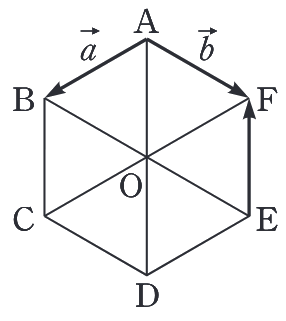
\includegraphics[width=\dmfigw]{figures/fig-153-308.png}\end{minipage}\par
